\documentclass[tikz]{standalone}

% \usepackage{newtxtext,newtxmath}

% mytikzset
\usepackage{tikz}
\usetikzlibrary{positioning,arrows,shapes}
\usetikzlibrary{decorations.pathmorphing}
\usetikzlibrary{decorations.markings}
\usetikzlibrary{shapes.arrows, fadings}
\usetikzlibrary{shapes,snakes}
\usetikzlibrary{calc}

\tikzset{
  vector/.style={thick,double,draw=black, postaction={decorate},
    decoration={markings,mark=at position .6 with {\arrow[black,scale=0.4]{triangle 45}}}},
  axial/.style={thick,double,densely dashed,draw=black, postaction={decorate},
    decoration={markings,mark=at position .6 with {\arrow[black,scale=0.4]{triangle 45}}}},
  gluon/.style={decorate, draw=black,
    decoration={coil,aspect=0.3,segment length=5pt,amplitude=3pt}},
  pseudo/.style={thick, dashed, draw=black, postaction={decorate},
    decoration={markings,mark=at position .6 with {\arrow[red,scale=0.5]{triangle 45}}}},
  scalar/.style={thick,draw=black, postaction={decorate},
    decoration={markings,mark=at position .6 with {\arrow[black,scale=0.5]{triangle 45}}}}%,
  % pomeron/.style={thick,draw=black, postaction={decorate},
  % decoration={zigzag,segment length=4,amplitude=.9}}
}

\definecolor{myGreen}{RGB}{0,127,0}

\begin{document}
\nopagecolor
  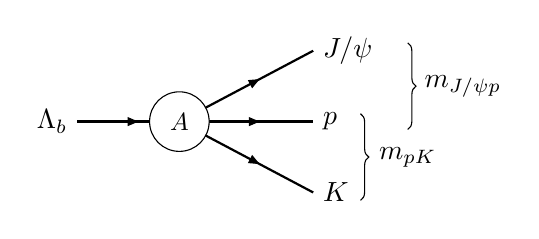
\begin{tikzpicture}[node distance=0.9cm and 1.3cm, baseline=1cm]
    \coordinate[] (c0);
    \coordinate[left=of c0,label= left:{$\Lambda_b$}] (Lamc);
    \coordinate[above right=of c0, xshift=4mm, label=right:{$J/\psi$}] (p);
    \coordinate[      right=of c0, xshift=4mm, label=right:{$p$}] (pi);
    \coordinate[below right=of c0, xshift=4mm, label=right:{$K$}] (K);

    \draw[scalar]  (Lamc) -- (c0);
    \draw[scalar]  (c0)   -- (p);
    \draw[scalar]  (c0)   -- (pi);
    \draw[scalar]  (c0)   -- (K);

    \draw[black, fill=white] (c0) circle (2.5ex) node[scale=0.9] {$A$};

    \draw [decorate,decoration={brace,amplitude=3pt}] ($(p)+(1.2,0.1)$) -- ($(pi)+(1.2,-0.1)$) node [black,midway,xshift=0.7cm] {$m_{J/\psi p}$};
    \draw [decorate,decoration={brace,amplitude=3pt}] ($(pi)+(0.6,0.1)$) -- ($(K)+(0.6,-0.1)$) node [black,midway,xshift=0.6cm] {$m_{pK}$};
    % \draw [decorate,decoration={brace,amplitude=3pt}] ($(b4)+(2.0,0.1)$) -- ($(b5)+(2.0,-0.1)$) node [black,midway,xshift=0.4cm] {$s$};
    % \draw [decorate,decoration={brace,amplitude=3pt}] ($(a1)-(1.5,0.1)$) -- ($(b1)-(1.2,-0.1)$) node [black,midway,xshift=-0.4cm] {$s_0$};

  \end{tikzpicture}
\end{document}
